% *********************************************************************
% © 2021-2023 Jeremy Sylvestre
%
% Permission is granted to copy, distribute and/or modify this document
% under the terms of the GNU Free Documentation License, Version 1.3 or
% any later version published by the Free Software Foundation; with no
% Invariant Sections, no Front-Cover Texts, and no Back-Cover Texts. A
% copy of the license is included in the appendix entitled “GNU Free
% Documentation License” that appears in the output document of this
% PreTeXt source code. All trademarks™ are the registered® marks of
% their respective owners.
%
% *********************************************************************

\newcommand*{\xmin}{-0.5}
\newcommand*{\xmax}{4.5}
\newcommand*{\ymin}{-0.25}
\newcommand*{\ymax}{1}

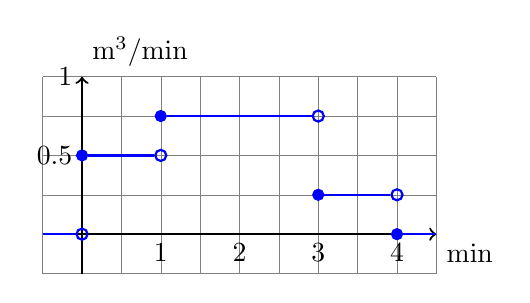
\begin{tikzpicture}
[
	closedpt/.style={circle,draw,fill,inner sep=0pt,minimum size=4pt},
	openpt/.style={circle,draw,inner sep=0pt,minimum size=4pt},
	yscale=2
]

	% grid
	\foreach \x in {-0.5,0,0.5,...,4.5} {
		\draw[very thin,gray] (\x,\ymin) -- (\x,\ymax);
	}
	\foreach \y in {-0.25,0,0.25,...,1} {
		\draw[very thin,gray] (\xmin,\y) -- (\xmax,\y);
	}

	% label grid
	\foreach \x in {1,2,3,4} {
		\node[below] at (\x,0) {$\x$};
	}
	\foreach \y in {0.5,1} {
		\node[left] at (0,\y) {$\y$};
	}

	% axes
	\draw[->,thick] (\xmin,0) -- (\xmax,0) node[below right] {min};
	\draw[->,thick] (0,\ymin) -- (0,\ymax) node[above right] {$\mathrm{m}^3/\mathrm{min}$};

	% off
	\node[blue,thick,openpt] at (0,0) (stop) {};
	\draw[blue,thick] (\xmin,0) -- (stop);

	% medium
	\node[blue,closedpt] at (0,0.5) (start) {};
	\node[blue,thick,openpt] at (1,0.5) (stop) {};
	\draw[blue,thick] (start) -- (stop);

	% high
	\node[blue,closedpt] at (1,0.75) (start) {};
	\node[blue,thick,openpt] at (3,0.75) (stop) {};
	\draw[blue,thick] (start) -- (stop);

	% low
	\node[blue,closedpt] at (3,0.25) (start) {};
	\node[blue,thick,openpt] at (4,0.25) (stop) {};
	\draw[blue,thick] (start) -- (stop);

	% off
	\node[blue,closedpt] at (4,0) (start) {};
	\draw[blue,thick] (start) -- (\xmax,0);

\end{tikzpicture}
